\documentclass{dtk}

\usepackage[utf8]{inputenc}
\usepackage[T1]{fontenc}
\usepackage{booktabs}
\usepackage{babel}
\usepackage{graphicx}
\usepackage{csquotes}
\usepackage{paralist}
\usepackage{xcolor}
\usepackage{microtype}

%\usepackage{mdframed} % Boxen
%\newmdenv [linecolor=black,backgroundcolor=gray!15, frametitle={Punktverteilung},leftmargin=1cm,rightmargin=1cm]{infobox}

\title{Wie man einen eigenen \TeX~Live Mirror aufsetzt}
\Author{Uwe}{Ziegenhagen}{Köln}

\definecolor{hellgelb}{rgb}{1,1,0.8}
\definecolor{lightgelb}{rgb}{1,1,0.8}
\definecolor{colKeys}{rgb}{0,0,1}
\definecolor{colIdentifier}{rgb}{0,0,0}
\definecolor{colComments}{rgb}{1,0,0}
\definecolor{colString}{rgb}{0,0.5,0}

\lstset{%
    float=hbp,%
    basicstyle=\ttfamily\footnotesize, %
    identifierstyle=\color{colIdentifier}, %
    keywordstyle=\color{colKeys}, %
    stringstyle=\color{colString}, %
    commentstyle=\color{colComments}, %
	language= Python,%
    columns=flexible, %
    tabsize=2, %
    morekeywords={fillwithlines, fillwithdottedlines,makeemptybox,part, fillwithgrid,answerline,gradetable,newmdenv,punkte,pointpoints},%
    morekeywords={bonuspointpoints,solutiontitle,chqword,chpgword,chpword,chbpword,chsword,chtword},%
    morekeywords={question,runningheadrule,firstpageheader,runningheader,dozent,fach,firstpagefooter,runningfooter,numpages},%
    morekeywords={choice,CorrectChoice,hpword,hsword,hqword,htword,firstpageheadrule},
    frame=single, %
    extendedchars=true, %
    showspaces=false, %
    showstringspaces=false, %
    numbers=left, %
    numberstyle=\tiny, %
    breaklines=true, %
    backgroundcolor=\color{yellow!15}, %
    breakautoindent=true, %
    captionpos=b%
}


\lstset{literate=%
    {Ö}{{\"O}}1
    {Ä}{{\"A}}1
    {Ü}{{\"U}}1
    {ß}{{\ss}}1
    {ü}{{\"u}}1
    {ä}{{\"a}}1
    {ö}{{\"o}}1
    {~}{{\textasciitilde}}1
}



\begin{document}

\maketitle

\begin{abstract}
In diesem Artikel möchte ich zeigen, wie man ein Netzwerkspeichersystem -- auch \enquote{NAS} genannt -- dazu benutzen kann, einen eigenen \TeX Live Spiegelserver für den Gebrauch im heimischen Netzwerk aufzusetzen.
\end{abstract}

\section{Einführung}

Als sehr \enquote{IT-affiner} Mensch geht es mir wie sicherlich vielen anderen Mitgliedern von Dante e.\,V. auch: ich habe zuhause (weit) mehr als einen Rechner. Und natürlich soll jeder dieser Rechner mit aktuellem \TeX Live ausgestattet sein. Selbstverständlich ließe sich jeder Rechner über einen der öffentlichen CTAN-Server aktuell halten, ein eigener Server innerhalb des lokalen Netzes bietet aber einige Vorteile: erstens verringert man dadurch sowohl die Last auf den CTAN-Servern, zweitens ist bei den meisten \TeX-Nutzern das interne Netzwerk noch immer deutlich schneller sein als die externe Datenleitung. Als technische Basis für den Betrieb nutze ich ein NAS (\enquote{Networked Attached Storage}) der Firma Synology, das sowieso rund um die Uhr angeschaltet ist.

\section{Kleiner Exkurs: Netzwerkfestplatten}

NAS-Systeme sind grundsätzlich kleine eigenständige Rechner, die an das lokale Netzwerk angeschlossen sind und üblicherweise ausschließlich per Weboberfläche administriert werden, was je nach Anbieter mehr oder weniger komfortabel ist. Sie verfügen meist über mehr als eine Festplatte, die über ein RAID zusammengeschlossen sind und Schutz gegen Datenausfall bieten sollen. Ein Einwurf an dieser Stelle sei noch erlaubt: ein RAID ersetzt kein Backup! Im Falle eines defekten RAID-Controllers sind die Daten auf allen Platten futsch, auch bei Diebstahl oder Wasser-/Feuerschaden nutzt die Redundanz durch das RAID nur wenig.

Zusammen mit der Firma QNAP ist Synology einer der Premiumhersteller, deren qualitativ sehr gute Geräte neben der eigentlichen Funktion eines Dateiservers noch viele andere Funktionen übernehmen können. 
Dem interessierten Leser sei die die Herstellerwebseite \url{www.synology.de} empfohlen. 

\section{Schritt 1: Aktivierung der \enquote{Webstation}}

Um später dem \TeX Live-Manager eine URL anbieten zu können, von der die Pakete geladen werden können, installieren und aktivieren wir im ersten Schritt die sogenannte \enquote{Webstation}, die nichts anderes ist als ein Apache Webserver mit PHP-Unterstützung.

\begin{figure}
\fbox{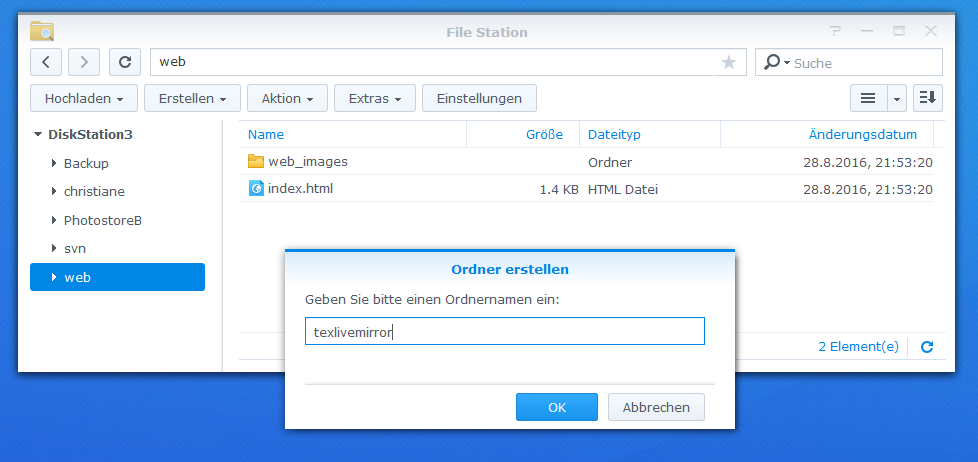
\includegraphics[width=\textwidth]{Ordner}}
\caption{Anlage des Unterordners \enquote{texlivemirror} im \enquote{web}-Ordner}\label{fig:Ordner}
\end{figure}

Das Installationspaket findet man im Paket-Zentrum, nach der Installation gibt es einen neuen gemeinsamen Ordner \texttt{web}, der alle Webserver-Inhalte aufnimmt. Hier erstellen wir über die Weboberfläche einen neuen Ordner \enquote{texlivemirror}, in dem die Daten später abgelegt werden (Abbildung \ref{fig:Ordner}).

\section{Schritt 2: Erstellung des \texttt{rsync}-Skripts}

Für den Abgleich zwischen entferntem und lokalem Datenstand nutze ich \texttt{rsync}, ein seit langer Zeit bewährtes Programm zur Synchronisation von Dateien und Verzeichnissen. Anhand des Vergleichs von Größe und Zeitstempel gleicht \texttt{rsync} nur die Dateien ab, die sich seit der letzten Synchronisation geändert haben.

Um das \texttt{rsync}-Skript zu erstellen, wird in unserem \enquote{web} Stammordner eine Datei \verb|update_texlive.sh| angelegt, die mit dem Inhalt aus Listing \ref{lis:rsync} befüllt wird. Die einzelnen Parameter des \texttt{rsync}-Aufrufs sind dabei:

\begin{description}
\item[a] fasst diverse Optionen für Unterverzeichnisse, symbolische Links und Rechte zusammen\footnote{Siehe beispielsweise \url{https://wiki.ubuntuusers.de/rsync/}}
\item[v] zeigt während der Synchronisation die ausgeführten Schritte an
\item [rsync://...] Die Quelle von der abgeglichen wird
\item [/volume1/...] Das abzugleichende lokale Zielverzeichnis
\end{description}

Da ich persönlich keine Möglichkeit gefunden habe, diese Datei anschließend über die Web-Oberfläche des NAS zu einem ausführbaren Skript zu machen, loggen wir uns als mit dem \texttt{admin}-Account des NAS darauf ein (der \texttt{ssh} Dienst -- den man in der Systemsteuerung unter \enquote{Terminal \& SNMP} aktiviert -- muss dazu laufen) und wechseln in den entsprechenden Ordner (\texttt{cd /volume1/web/}). Ein anschließendes \verb|chmod +x update_texlive.sh| setzt das entsprechende execute-Flag.

\begin{lstlisting}[label={lis:rsync},caption={\texttt{update\textunderscore texlive.sh}, das \texttt{rsync} Skript für die Synchronisation}]
rsync -av rsync://rsync.dante.ctan.org/CTAN/systems/texlive/tlnet/ /volume1/web/texlivemirror/
\end{lstlisting}

Jetzt können wir das Skript bereits aufrufen und den initialen Datenstand vom entfernten Server holen. Listing \ref{lis:job} zeigt die ersten Zeilen des Skript-Aufrufs.

\begin{lstlisting}[label={lis:job},caption={Die ersten Output-Zeilen des ersten Skript-Aufrufs}]
admin@DiskStation3:/volume1/web$ ./update_texlive.sh

receiving incremental file list
./
archive/
archive/12many.doc.tar.xz
archive/12many.source.tar.xz
archive/12many.tar.xz
archive/2up.doc.tar.xz
archive/2up.tar.xz
archive/Asana-Math.doc.tar.xz
archive/Asana-Math.tar.xz
archive/ESIEEcv.doc.tar.xz
archive/ESIEEcv.source.tar.xz
archive/ESIEEcv.tar.xz
archive/FAQ-en.doc.tar.xz
archive/FAQ-en.tar.xz
archive/GS1.doc.tar.xz
\end{lstlisting}


\section{Automatischer Aufruf}

Damit sich unser \TeX-Spiegelserver die jeweils neuesten Inhalte beschaffen zeitgesteuert holen soll, müssen wir nun dafür sorgen, dass das Skript regelmäßig aufgerufen wird. Was auf einer normalen Unix/Linux Maschine der \texttt{cronjob} ist, ist auf dem Synology NAS der Aufgabenplaner in der Systemsteuerung, siehe Abbildung \ref{fig:tasks}.

Hier erstellen wir über die drei Tabs (siehe Abbildungen \ref{fig:task1} bis \ref{fig:task2}) einen neuen Task, der im Beispiel täglich um 01:00 Uhr nachts das Update-Skript aufruft.

\begin{figure}
\begin{center}
\fbox{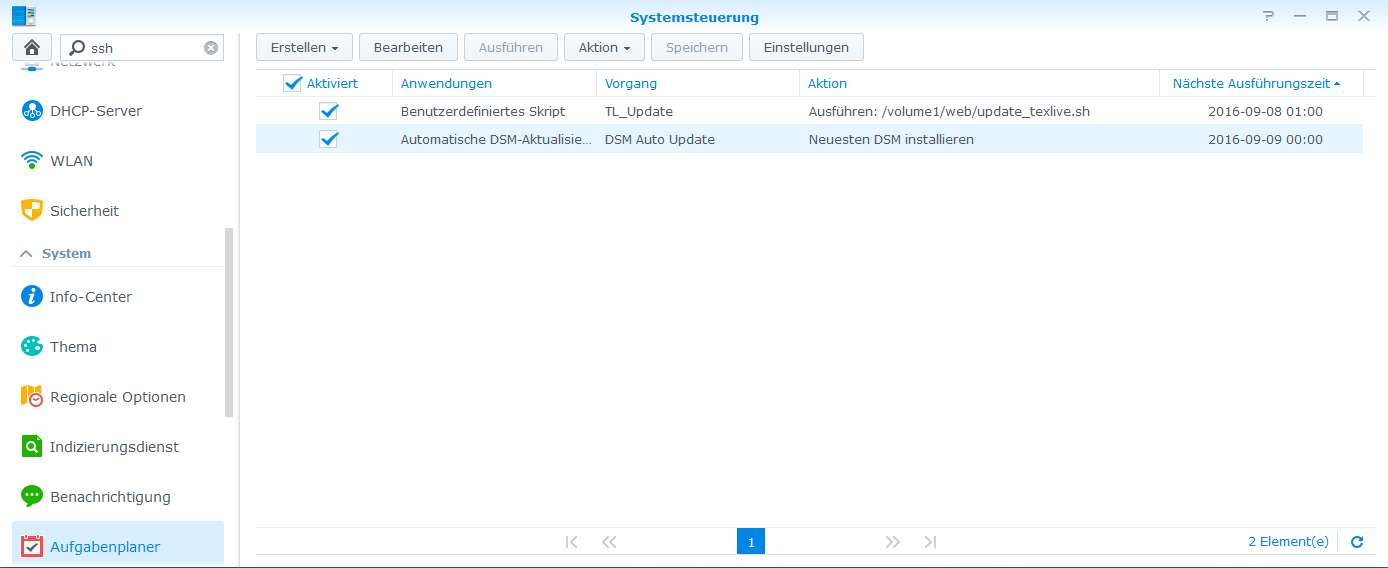
\includegraphics[width=0.9\textwidth]{Systemsteuerung}}
\caption{Der Aufgabenplaner in der Systemsteuerung}\label{fig:tasks}
\end{center}
\end{figure}

\begin{figure}
\begin{center}
\fbox{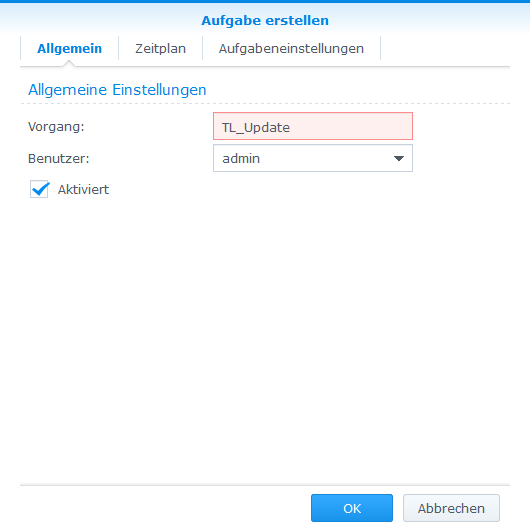
\includegraphics[width=0.45\textwidth]{Task1}}
\fbox{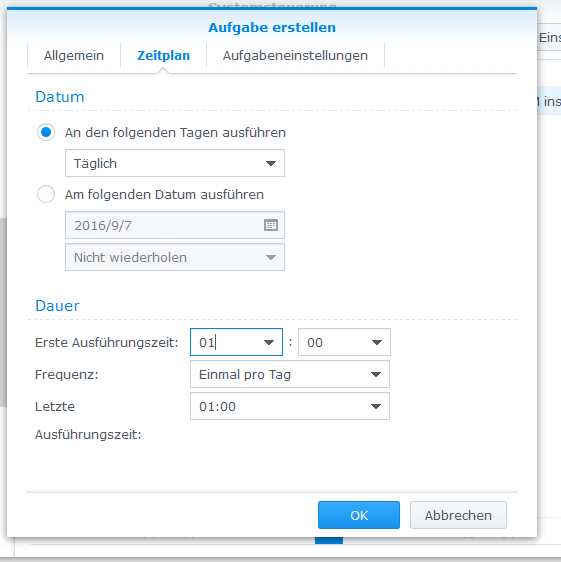
\includegraphics[width=0.45\textwidth]{Task2}}
\caption{Die Tabs \enquote{Allgemein} und \enquote{Aufgabe erstellen} der neuen Aufgabe}\label{fig:task1}
\end{center}
\end{figure}

\begin{figure}
\begin{center}
\fbox{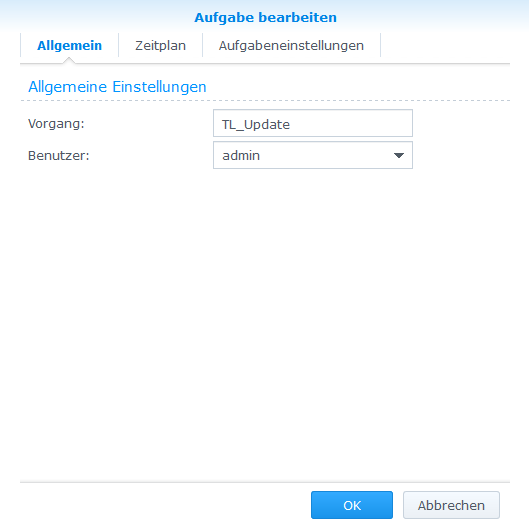
\includegraphics[width=0.55\textwidth]{Task3}}
\caption{Der Tab \enquote{Aufgabeneinstellungen} der neuen Aufgabe}\label{fig:task2}
\end{center}
\end{figure}

\section{Installation und Update mit dem eigenen Server}

Bei einer Neu-Installation von \TeX~Live müssen wir jetzt nicht mehr das Install-Skript von \url{http://tug.org/texlive} holen, sondern könnten es über den Webbrowser von unserem NAS unter \url{http://<IP-Adresse_des_NAS>/texlivemirror/} herunterladen. Jedoch fehlt noch ein Schritt, denn in der Standardkonfiguration listet die Webstation das Verzeichnis nicht auf, sondern liefert den Fehler 403 zurück. Es fehlt noch eine \texttt{.htaccess} Datei im \texttt{texlivemirror} Verzeichnis. Auch wenn ich persönlich Emacs bevorzuge, an dieser Stelle tut es -- mangels installiertem Emacs -- auch \texttt{vi}: wir loggen uns wieder per SSH ein, wechseln nach \texttt{/volume1/web/texlivemirror} und geben den Befehl \texttt{vi .htaccess} ein. Im \texttt{vi} nutzen wir die Taste \enquote{i}, um in den Einfügemodus zu kommen und geben dann \texttt{Options +Indexes} ein. Mit \texttt{<Escape> :wq} speichern wir und beenden \texttt{vi}.\footnote{Mehr als die drei oder vier Tastenkombinationen werde ich mir persönlich nie merken können\ldots} 

Anschließend starten wir das Installations-Skript mittels (unter Windows)  

{\footnotesize \verb|install-tl-windows.bat --location http://<IP-Adresse_des_NAS>/texlivemirror/|} 

beziehungsweise (unter Linux/Unix) 

{\footnotesize \verb|install-tl --location http://<IP-Adresse_des_NAS>/texlivemirror/|}

um \TeX~Live den neuen Spiegelserver bekannt zu machen. Nach der \TeX~Live Installation setzt man dann nur noch das Standard-Repository mittels 

\verb|tlmgr option repository http://<IP-Adresse_des_NAS>/texlivemirror|

\section{Fazit}

Der Artikel hat am Beispiel eines Synology NAS gezeigt, wie man mit vergleichsweise wenig Aufwand einen eigenen Spiegelserver aufsetzen kann, um das lokale Netzwerk schnell und bequem mit \TeX Live Updates zu versorgen. Das gezeigte Vorgehen lässt sich leicht auf andere Umgebungen übertragen, auch ein Raspberry Pi könnte die Aufgabe leicht übernehmen.

Für Kommentare, Anregungen und Ergänzungen bin ich jederzeit dankbar.
\end{document}